\documentclass[twoside]{article}
\setlength{\oddsidemargin}{0.25 in}
\setlength{\evensidemargin}{-0.25 in}
\setlength{\topmargin}{-0.6 in}
\setlength{\textwidth}{6.5 in}
\setlength{\textheight}{8.5 in}
\setlength{\headsep}{0.75 in}
\setlength{\parindent}{0 in}
\setlength{\parskip}{0.1 in}

\usepackage{graphicx}
\usepackage{url}

% For alignment
\usepackage{ragged2e}


% For fancy arrows
\usepackage{tikz}
\usetikzlibrary{fadings,shapes.arrows,shadows}
\usepackage{xparse}
\usepackage{lipsum}
\tikzfading[name=arrowfading, top color=transparent!0, bottom color=transparent!95]
\tikzset{arrowfill/.style={#1,general shadow={fill=black, shadow yshift=-0.8ex, path fading=arrowfading}}}
\tikzset{arrowstyle/.style n args={3}{draw=#2,arrowfill={#3}, single arrow,minimum height=#1, single arrow,
single arrow head extend=.3cm,}}
\NewDocumentCommand{\tikzfancyarrow}{O{2cm} O{FireBrick} O{top color=OrangeRed!20, bottom color=Red} m}{
\tikz[baseline=-0.5ex]\node [arrowstyle={#1}{#2}{#3}] {#4};
}

%
% The following commands sets up the lecnum (lecture number)
% counter and make various numbering schemes work relative
% to the lecture number.
%
\newcounter{lecnum}
\renewcommand{\thepage}{\thelecnum-\arabic{page}}
\renewcommand{\thesection}{\thelecnum.\arabic{section}}
\renewcommand{\theequation}{\thelecnum.\arabic{equation}}
\renewcommand{\thefigure}{\thelecnum.\arabic{figure}}
\renewcommand{\thetable}{\thelecnum.\arabic{table}}
\newcommand{\dnl}{\mbox{}\par}

%
% The following macro is used to generate the header.
%
\newcommand{\lecture}[4]{
  \pagestyle{myheadings}
  \thispagestyle{plain}
  \newpage
  \setcounter{lecnum}{#1}
  \setcounter{page}{1}
  \noindent
  \begin{center}
  \framebox{
     \vbox{\vspace{2mm}
   \hbox to 6.28in { {\bf COMPSCI~630~~~Systems
                       \hfill Spring 2018} }
      \vspace{4mm}
      \hbox to 6.28in { {\Large \hfill Lecture #1: #2  \hfill} }
      \vspace{2mm}
      \hbox to 6.28in { {\it Lecturer: #3 \hfill Scribe(s): #4} }
     \vspace{2mm}}
  }
  \end{center}
  \markboth{Lecture {#1}: #2}{Lecture {#1}: #2}
  \vspace*{4mm}
}

%
% Convention for citations is authors' initials followed by the year.
% For example, to cite a paper by Leighton and Maggs you would type
% \cite{LM89}, and to cite a paper by Strassen you would type \cite{S69}.
% (To avoid bibliography problems, for now we redefine the \cite command.)
%
\renewcommand{\cite}[1]{[#1]}

% \input{epsf}

%Use this command for a figure; it puts a figure in wherever you want it.
%usage: \fig{NUMBER}{FIGURE-SIZE}{CAPTION}{FILENAME}
\newcommand{\fig}[4]{
           \vspace{0.2 in}
           \setlength{\epsfxsize}{#2}
           \centerline{\epsfbox{#4}}
           \begin{center}
           Figure \thelecnum.#1:~#3
           \end{center}
   }

% Use these for theorems, lemmas, proofs, etc.
\newtheorem{theorem}{Theorem}[lecnum]
\newtheorem{lemma}[theorem]{Lemma}
\newtheorem{proposition}[theorem]{Proposition}
\newtheorem{claim}[theorem]{Claim}
\newtheorem{corollary}[theorem]{Corollary}
\newtheorem{definition}[theorem]{Definition}
\newenvironment{proof}{{\bf Proof:}}{\hfill\rule{2mm}{2mm}}

% Some useful equation alignment commands, borrowed from TeX
\makeatletter
\def\eqalign#1{\,\vcenter{\openup\jot\m@th
 \ialign{\strut\hfil$\displaystyle{##}$&$\displaystyle{{}##}$\hfil
     \crcr#1\crcr}}\,}
\def\eqalignno#1{\displ@y \tabskip\@centering
 \halign to\displaywidth{\hfil$\displaystyle{##}$\tabskip\z@skip
   &$\displaystyle{{}##}$\hfil\tabskip\@centering
   &\llap{$##$}\tabskip\z@skip\crcr
   #1\crcr}}
\def\leqalignno#1{\displ@y \tabskip\@centering
 \halign to\displaywidth{\hfil$\displaystyle{##}$\tabskip\z@skip
   &$\displaystyle{{}##}$\hfil\tabskip\@centering
   &\kern-\displaywidth\rlap{$##$}\tabskip\displaywidth\crcr
   #1\crcr}}
\makeatother

% **** IF YOU WANT TO DEFINE ADDITIONAL MACROS FOR YOURSELF, PUT THEM HERE:



% Some general latex examples and examples making use of the
% macros follow.

\begin{document}

%FILL IN THE RIGHT INFO.
%\lecture{**LECTURE-NUMBER**}{**DATE**}{**LECTURER**}{**SCRIBE**}
\lecture{2}{Compilation, FORTRAN, and LISP}{Emery Berger}{Sarthak Nandi}

\section{Last Class}

FORTRAN and COBOL - FORTRAN was for scientists, COBOL was for business people

\section{Grammar and Parsing}

Chomsky hierarchy (1956):

\begin{center}
    Recursively enumerable

    \tikzfancyarrow[1cm][top color= PaleTurquoise,bottom color=DeepSkyBlue,shape border rotate=90]{} % Errors, but works

    Context sensitive
    
    \tikzfancyarrow[1cm][top color= PaleTurquoise,bottom color=DeepSkyBlue,shape border rotate=90]{}
    
    Context free (CFG)
    
    \tikzfancyarrow[1cm][top color= PaleTurquoise,bottom color=DeepSkyBlue,shape border rotate=90]{}
    
    Reg exps
\end{center}

We talk about grammar in "production style" from Algol-60 - Backus-Naur form (BNF)

\hspace{1cm}expr ::= '(' expr ')' $|$ number $|$ expr op expr $|$ unary op expr

People have stopped working on parsing now.

backtracking $~$ exponential time

N tokens $2^N$

Keep tokens in memory - needs to be efficient - Symbol table

Text $->$ Lexer (e.g. Lex, Flex) $->$ Tokens $->$ Parser (insert grammar) $->$ Parse LL(1) , yacc/bison (LALR(1)), Java - Antlr

Packrat parsing - backtracking parser, general enough to handle things like C preprocessor \#define

Newer PL don't have such things, macros are discouraged because you can do things like:

\hspace{1cm}\#define while if

\section{Compiler Optimizations}

One of goals of FORTRAN: fast code. Invented field of compiler optimization

Requirement: preserve semantics

Code(P) \tikzfancyarrow[1cm]{Compiler} Assembly (P')

For all inputs: P(i) = P'(i)

Memory hierarchy:

Then: Registers, memory

Now: L0...L4, RAM

One problem: very few registers. So can keep some number of variables only in registers.

\begin{center}
    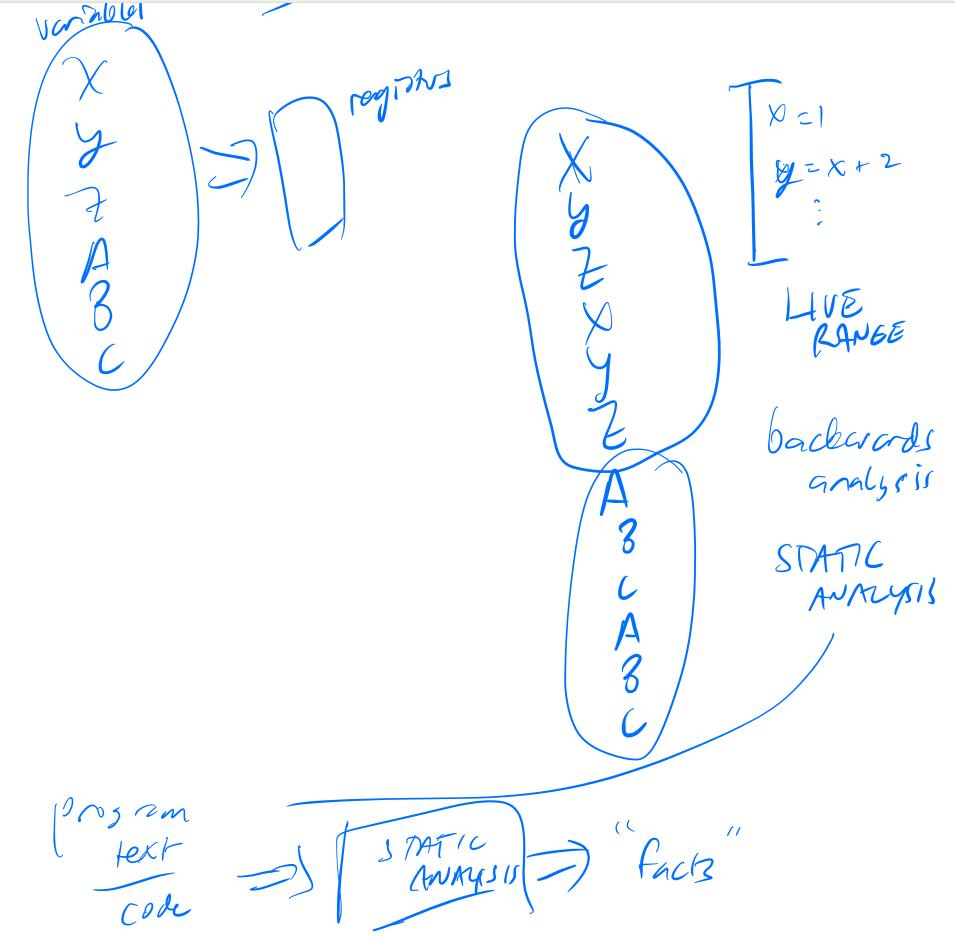
\includegraphics[scale=0.32]{live_range.jpg}
\end{center}

Good performance if number of variables in distinct live ranges is same as number of registers.

To find live range: backwards analysis, starting from bottom go up until you see the last use

First instance of static analysis:

Program text code \tikzfancyarrow[1cm]{Static Analysis} "facts"

Reality is subset of facts from static analysis.

\begin{center}
    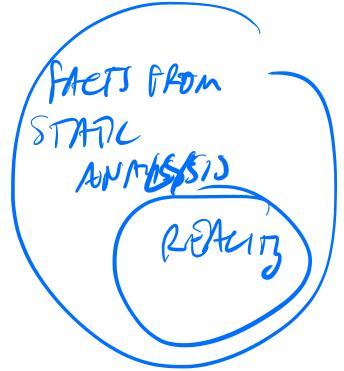
\includegraphics[scale = 0.32]{reality_subset.jpg}    
\end{center}

\textbf{Halting problem:} Given program P: for all i inputs : P(i) terminates.

Proof by contradiction:
\begin{verbatim}
    if halts(P)
        run forever
    else
        halt
\end{verbatim}
    
You can turn many complex analysis problems to halting problems, including static analysis for live range.

Basic static analysis on straight line code

Add complexity: Loops, Recursion, Pointers, Function calls, 1st class functions, EVAL (= EVIL) (Take string code and execute)

Intraprocedural: analyze within a function to optimize

Interprocedural: analyze whole program to optimize

(Why fortran is faster than C in next section)

Register allocation = graph coloring, NP complete problem.

\textbf{Strength reduction:} Replace an expensive operator by a cheaper one

X = pow(3,2) = ($3^2$) can be replaced by

X = 3*3 = 9

\textbf{Constant propagation:} Replace constant usages with constant value
Y = 12

X = Y+1 = 13

\textbf{Inlining:} Expand out some (small) functions in a program

\begin{verbatim}
    int add(int x, int y) {
        return x+y
    }

    foo() {
        int c = add(2,3) = 2+3 = 5
    }    
\end{verbatim}


Inlining effect is multiplied when function calls in loops are replaced. Inlining exposes optimization opportunities, reduces functional call overhead. Careful inlining combines with all optimizations

FORTRAN - optimizing compilation, LISP - interpreters

Starting in 90s we hybridised: JIT compiler

\textbf{Ski-rental problem (CLRS):} When you go skiing 1st time should you buy or rent equipment ? When should you buy ?
\begin{itemize}
    \item Rental: \$10, Purchase: \$100
    \item Renting too many times and then purchasing is a bad idea, purchasing and using only once is also a bad idea.
    \item Hybrid: rent once, then buy
    \item Optimal strategy: Rent until you spend \$100
    \itemWorst case: Spend \$200 when could have spent \$100.
\end{itemize}

Whole program analysis (with closed-world assumption): Big program would be slow

Modular analysis: C was designed for this, Go took this further. But can't determine how many times a function is called.

Real-time computation area - We need some deadline for real time systems.

JIT - Interpreter

Fast JIT - 00 (no optimization)

\hspace{1cm}- 01
    
\hspace{1cm}-02 (increasing optimization as we go down)
    
Modern JIT compilers will replace code within loops while it's in it if loop is long

(Paper by Jim Larus, repaying Moore)

LLVM is integrated in Safari for JS.

Compilers convert "dumb slow code" to "smart fast code", but can't replace algorithms.

\newpage

\subsection{Why FORTRAN is faster than C}

Alias analysis, pointer analysis don't exist in FORTRAN (mostly)

\begin{verbatim}
    X = [1,2,3] Y = [1,2,3]
    INT *X;     INT *Y
    FOR 
        X[i]    Y[i[]
        X+i     Y+i
        X=A     Y=B
    
    if ()
        X = Y <- Don't know what happens in this case
    else
        ..
    
\end{verbatim}

\section{Lisp}

\begin{itemize}
  \item Logical view of programming - Lambda calculus
  \item LISP is executable version of this logic, first functional PL (function-centric, functions are first class objects you can have list of function, can pass them)
  \item FORTRAN, COBOL are kinda hacks
  \item The code and data is same (homoiconicity)
  \item Compiler not needed - obviated
  \item Led to LISP being used for complex purposes
  \item Garbage collection
\end{itemize}


\end{document}
